\documentclass{article}
\usepackage[utf8]{inputenc}
\usepackage{graphicx} 
\renewcommand{\thefigure}{S\arabic{figure}}
\renewcommand{\thetable}{S\arabic{table}}
\usepackage[bottom=2cm,top=2cm, margin=2cm]{geometry}
\topmargin=-0.4in
\topmargin=-0.5in
\usepackage{imakeidx}
\makeindex[columns=3, title=Alphabetical Index, intoc]
\usepackage[round]{natbib} 
\bibliographystyle{plainnat}
\usepackage[T1]{fontenc}
\usepackage[T1]{fontenc}

\centering
\title{Supplementary Information}
\author{Kate Griffin}
\date{August 2022}

\begin{document}

\maketitle
\vspace*{4\baselineskip}
\tableofcontents
\clearpage
\tiny
\centering
\tiny
\section{\emph{E} Estimates}

\subsection{\emph{E} Estimates for Active vs Resting Metabolic Rate}

\begin{figure}[h]
    \centering
    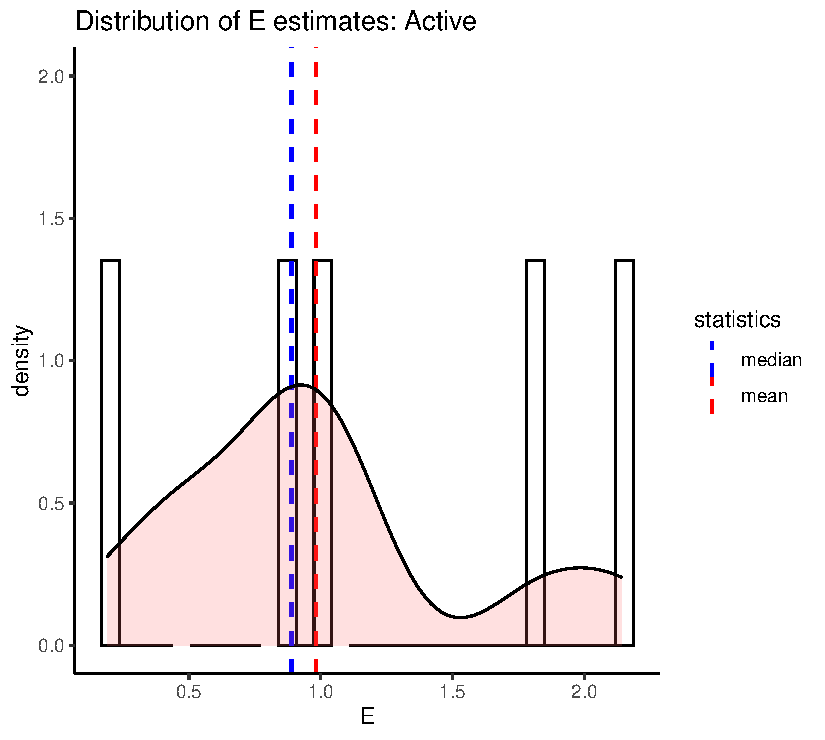
\includegraphics[width=6in]{active.pdf}
    \caption{\label{fig:S1} Distribution of \emph{$E$} estimates only for observations where metabolic rate was measured as Active Metabolic Rate (AMR). The mean is represented by the broken red line, and the median is represented by the broken blue line. No significant difference was found between AMR and RMR}
\end{figure}

\begin{figure}[h]
    \centering
    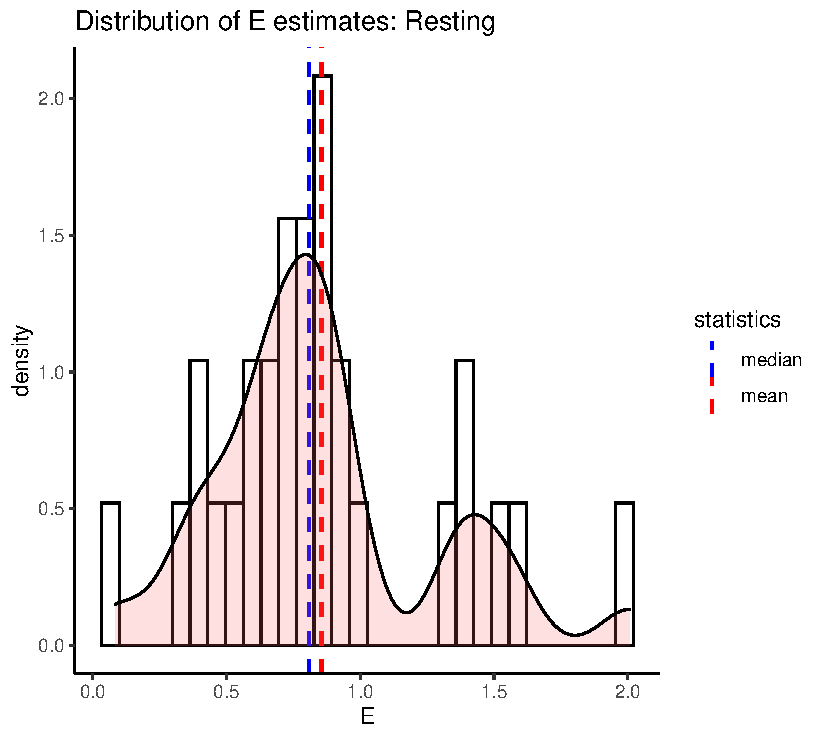
\includegraphics[width=6in]{resting.pdf}
    \caption{\label{fig:S2} Distribution of \emph{$E$} estimates only for observations where metabolic rate was measured as Resting Metabolic Rate (RMR). The mean is represented by the broken red line, and the median is represented by the broken blue line. No significant difference was found between RMR and AMR}
\end{figure}
\clearpage

\subsection{\emph{E} estimates for Juvenile vs Adult individuals}
\begin{figure}[h]
    \centering
    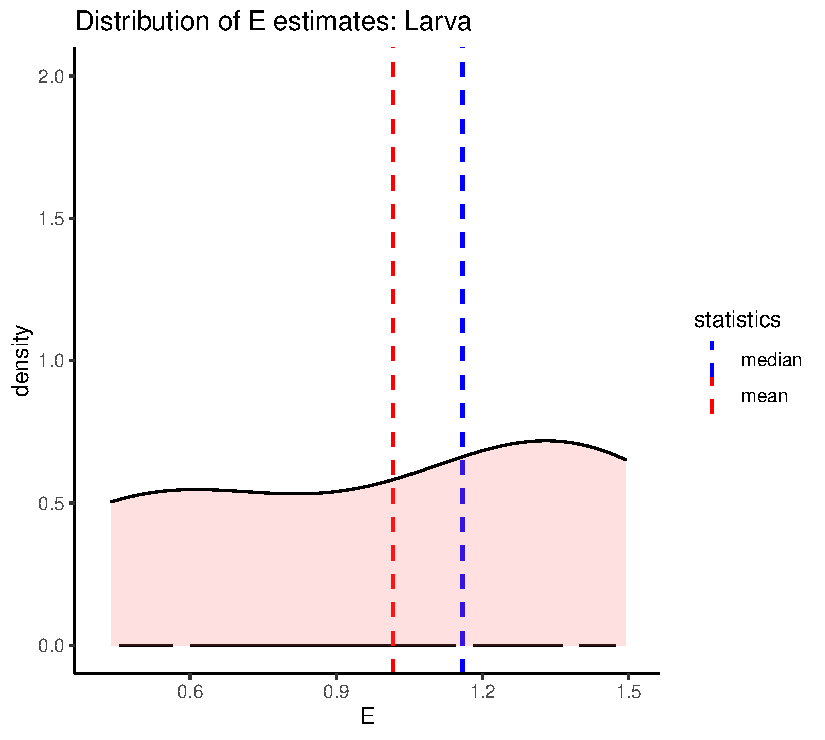
\includegraphics[width=6in]{larva.pdf}
    \caption{\label{fig:S3} Distribution of \emph{$E$} estimates for only juvenile individuals. The mean is represented by the broken red line, and the median is represented by the broken blue line. No significant difference was found between juveniles and adults}
\end{figure}

\begin{figure}[h]
    \centering
    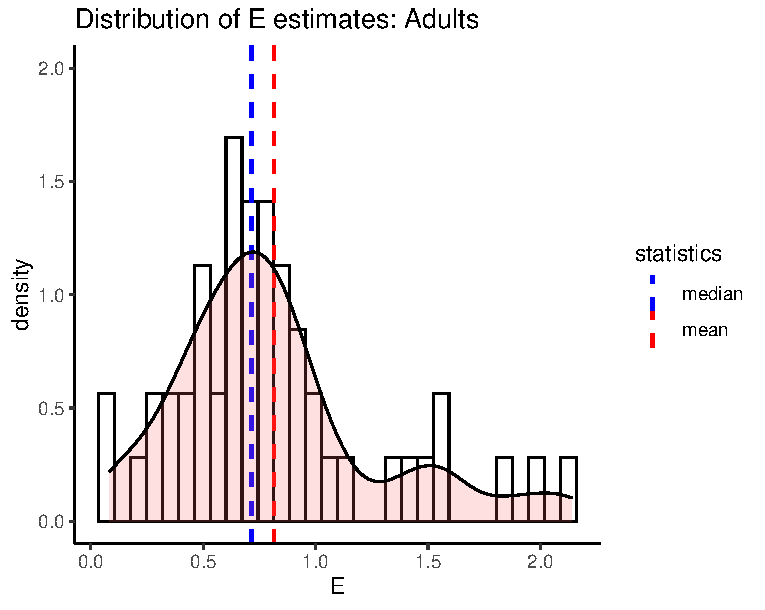
\includegraphics[width=6in]{adult.pdf}
    \caption{\label{fig:S4} Distribution of \emph{$E$} estimates for only adult individuals. The mean is represented by the broken red line, and the median is represented by the broken blue line. No significant difference was found between adults and juveniles}
\end{figure}

\clearpage
\begin{table}[h]
\centering
 \footnotesize
 \begin{tabular}{llll}
Species                         & E           & E SE        & R squared   \\
 \hline\hline
Bombus vosnesenskii             & 0.795995691 & 0.519513655 & 0.768640021 \\
Paractora dreuxi                & 0.492948089 & 0.851216137 & 0.919069276 \\
Antrops truncipennis            & 0.519733915 & 0.12602785  & 0.949899535 \\
Amara quenseli                  & 0.189969656 & 26.56378245 & 0.828858879 \\
Simplocaria metallica           & 1.018278908 & -           & 0.997071698 \\
Rhynchaenus flagellum           & 1.090823733 & 2.156076551 & 0.675770726 \\
Lycosa carolinensis             & 0.458168029 & 0.068119442 & 0.916614916 \\
Extatosoma tiaratum             & 0.354621452 & -           & 0.971776666 \\
Apis mellifera carnica          & 0.994649628 & -           & 0.96923159  \\
Nauphoeta cinerea               & 1.831636306 & 0.780667213 & 0.976736055 \\
Carcinus maenas                 & 2.021669833 & 0.797398154 & 0.921334173 \\
Glossina pallidipes             & 0.612657432 & 0.165002862 & 0.893011942 \\
Lithobius curtipes              & 1.577584106 & 0.891029051 & 0.997966087 \\
Lithobius mutabilis             & 1.40390885  & 1.245567932 & 0.998374122 \\
Hippodamia convergens           & 3.304312841 & 0.175938531 & 0.834119522 \\
Encoptolophus sordidus costalis & 0.096488088 & -           & 0.986257239 \\
Atta laevigata                  & 0.64706128  & 0.682273465 & 0.988949986 \\
Atta sexdens rubropilosa        & 0.717277783 & 0.270384912 & 0.990726469 \\
Melanoplus sanguinipes          & 0.634944867 & 1.289783243 & 0.983196815 \\
Trimerotropis pallidipennis     & 0.535033066 & 1.231336204 & 0.970151636 \\
Scarabaeus gariepinus           & 0.625501332 & 1.773276754 & 0.99823373  \\
Scarabaeus galenus              & 2.571994622 & 34.26935686 & 0.90918744  \\
Scarabaeus rusticus             & 0.809486625 & 0.000407649 & 0.999999978 \\
Scarabaeus westwoodi            & 0.410396951 & 0.123821896 & 0.983942731 \\
Scarabaeus hippocrates          & 0.930985417 & -           & 0.994743927 \\
Helius waitei                   & 0.713151711 & 5.217554261 & 0.911350848 \\
Pterohelaeus spp.               & 1.337872711 & 2.459757271 & 0.88450702  \\
Cerotalis spp.                  & 0.298707389 & 0.201197941 & 0.924093513 \\
Carenum spp.                    & 0.638414548 & -           & 0.979833195 \\
Solenopsis invicta              & 2.139951466 & 0.356189512 & 0.907601313 \\
Hydromedion sparsutum           & 1.581754853 & -           & 0.937387348 \\
Orchelimum fidicinium           & 0.274484614 & -           & 0.773202971 \\
Pogonomyrmex occidentalis       & 0.665393192 & 1.754747013 & 0.492760921 \\
Glossina morsitans orientalis   & 0.703865161 & 0.04459742  & 0.990186485 \\
Anurogryllus arboreus           & 1.523104973 & 3.331325564 & 0.952372553 \\
Oecanthus celerinictus          & 0.854619683 & 0.160350106 & 0.998971969 \\
Oecanthus quadripunctatus       & 0.53509874  & 0.306775497 & 0.996759376 \\
Pogonomyrmex maricopa           & 1.108836087 & -           & 0.981722437 \\
Aphaenogaster cockerelli        & 1.250221318 & -           & 1           \\
Camponotus vafer                & 1.171060813 & -           & 1           \\
Hophlosphyrum griseus           & 0.856565787 & 4.691078676 & 0.560136089 \\
Pleocoma australis              & 0.924353735 & 3.745589741 & 0.817055749 \\
Bootettix punctatus             & 0.811671409 & -           & 1           \\
Pachydiplax longipennis         & 0.684961168 & 0.723955555 & 0.991176653 \\
Trimrrotropis suffusa           & 2.005767452 & 0.533240686 & 0.924639446 \\
Cystosoma saundersii            & 0.852432901 & -           & 1           \\
Camponotus fulvopilosus         & 0.474979676 & 0.095955566 & 0.912478335 \\
Canonopsis sericeus             & 0.611634659 & -           & 0.99983965  \\
Palirhoeus eatoni               & 0.085343175 & -           & 0.985598162 \\
Bothrometopus randi             & 0.877997456 & -           & 0.99790676  \\
Ectemnorhinus marioni           & 0.713782039 & -           & 1           \\
Ectemnorhinus similis           & 0.567205605 & -           & 0.999998433 \\
Formica pratensis               & 0.796054362 & 0.811442609 & 0.988767856 \\
Neophilaenus lineatus           & 0.775596808 & -           & 1           \\
Diceroprocta apache             & 0.921143865 & 0.787115087 & 0.997090503 \\
Xenopsylla ramesis              & 0.38907     & 0.237067565 & 0.826486082 \\
Pogonomyrmex rugosus            & 0.487265603 & 0.076805881 & 0.817923862 \\
Messor capitatus                & 0.888714102 & 1.509267874 & 0.910655578 \\
Cydia pomonella                 & 1.492993509 & 12.76560293 & 0.981465908 \\
Limnephilus rhombicus           & 0.438572259 & 0.050783072 & 0.952581951 \\
Glossina morsitans centralis    & 1.394348932 & -           & 0.998847755 \\
Glossina morsitans morsitans    & 1.159390825 & 8.377314878 & 0.730596403 \\
Alphitobius diaperinus          & 0.598233005 & 2.467036709 & 0.958259648
\end{tabular}

\caption{\label{Table:S3} \emph{$E$} values calculated for each individual species. Values were estimated by fitting a four-parameter adaptation of the Sharpe-Schoolfield model \citep{kontopoulos2020adaptive} to each subset of data. Values for $R^2$ and standard error (SE) for \emph{E} are also provided}
\end{table}
\clearpage

\section{Residuals vs Fitted values}
\subsection{\emph{E} $\sim$ Latitude}
\begin{figure}[h]
    \centering
    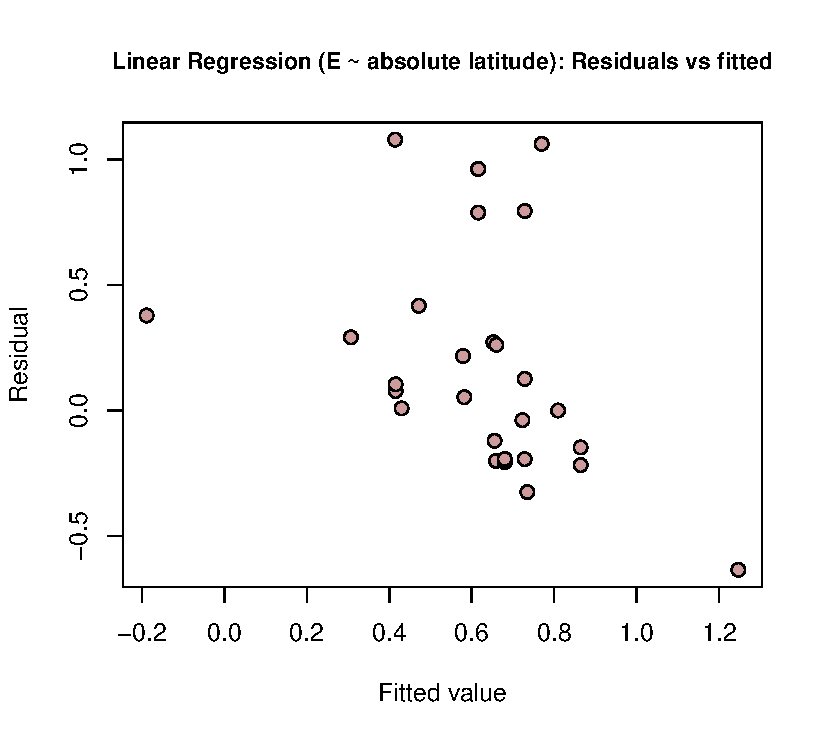
\includegraphics[width=3.5in]{Lat_lin_rs.pdf}
    \caption{\label{fig:S5} Residual vs fitted value for \emph{E} $\sim$ |latitude| linear model}
\end{figure}
\begin{figure}[h]
    \centering
    \includegraphics[width=3.5in]{Lat_poly_rs.pdf}
    \caption{\label{fig:S6} Residual vs fitted value for \emph{E} $\sim$ Latitude polynomial model}
\end{figure}
\clearpage

\subsection{\emph{E} $\sim$ Size}
\begin{figure}[h]
    \centering
    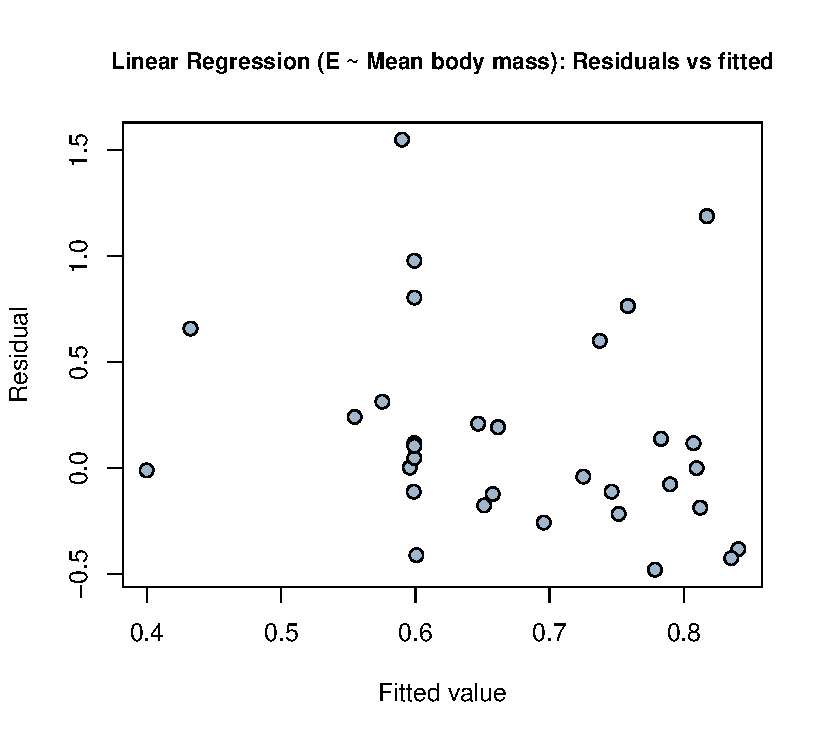
\includegraphics[width=3.5in]{L_size_rs.pdf}
    \caption{\label{fig:S7} Residual vs fitted value for \emph{E} $\sim$ Size linear model}
\end{figure}
\begin{figure}[h]
    \centering
    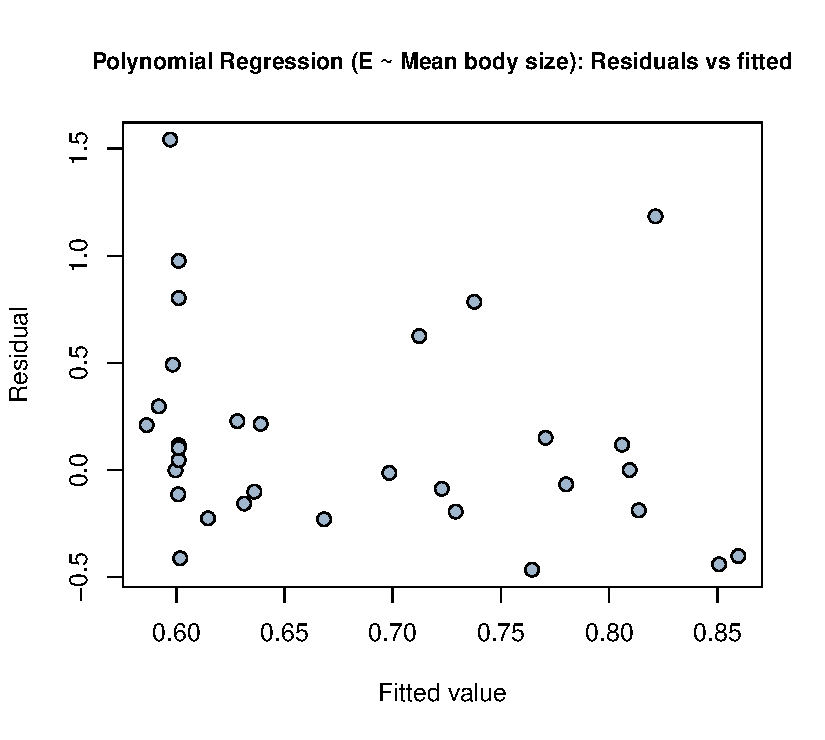
\includegraphics[width=3.5in]{p_size_rs.pdf}
    \caption{\label{fig:S8} Residual vs fitted value for \emph{E} $\sim$ Size polynomial model}
\end{figure}
\clearpage

\subsection{\emph{E} $\sim$ Latitude $\times$ Size}
\begin{figure}[h]
    \centering
    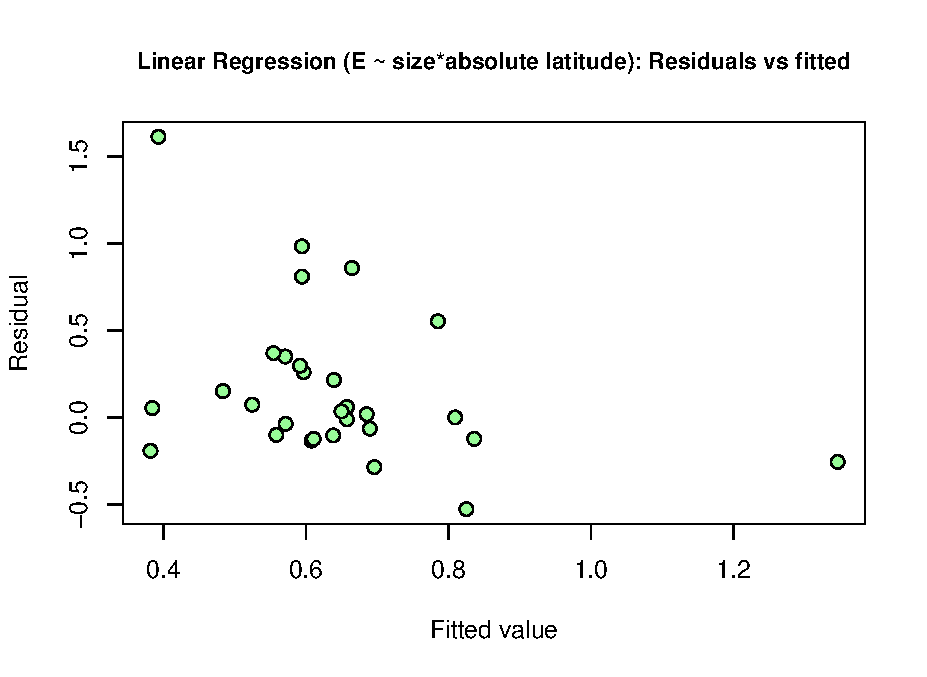
\includegraphics[width=3.5in]{1.pdf}
    \caption{\label{fig:S9} Residual vs fitted value for \emph{E} $\sim$ Latitude $times$ Size linear model}
\end{figure}
\begin{figure}[h]
    \centering
    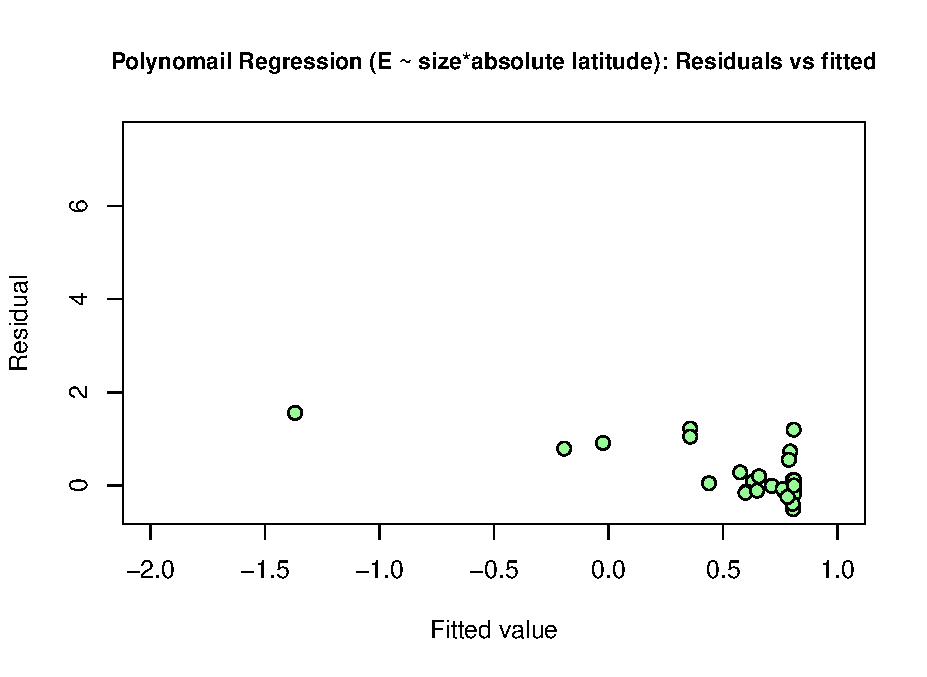
\includegraphics[width=3.5in]{2.pdf}
    \caption{\label{fig:S10} Residual vs fitted value for \emph{E} $\sim$ Size polynomial model}
\end{figure}
\clearpage

\section{Metabolic Rates}
\begin{figure}[h]
    \centering
    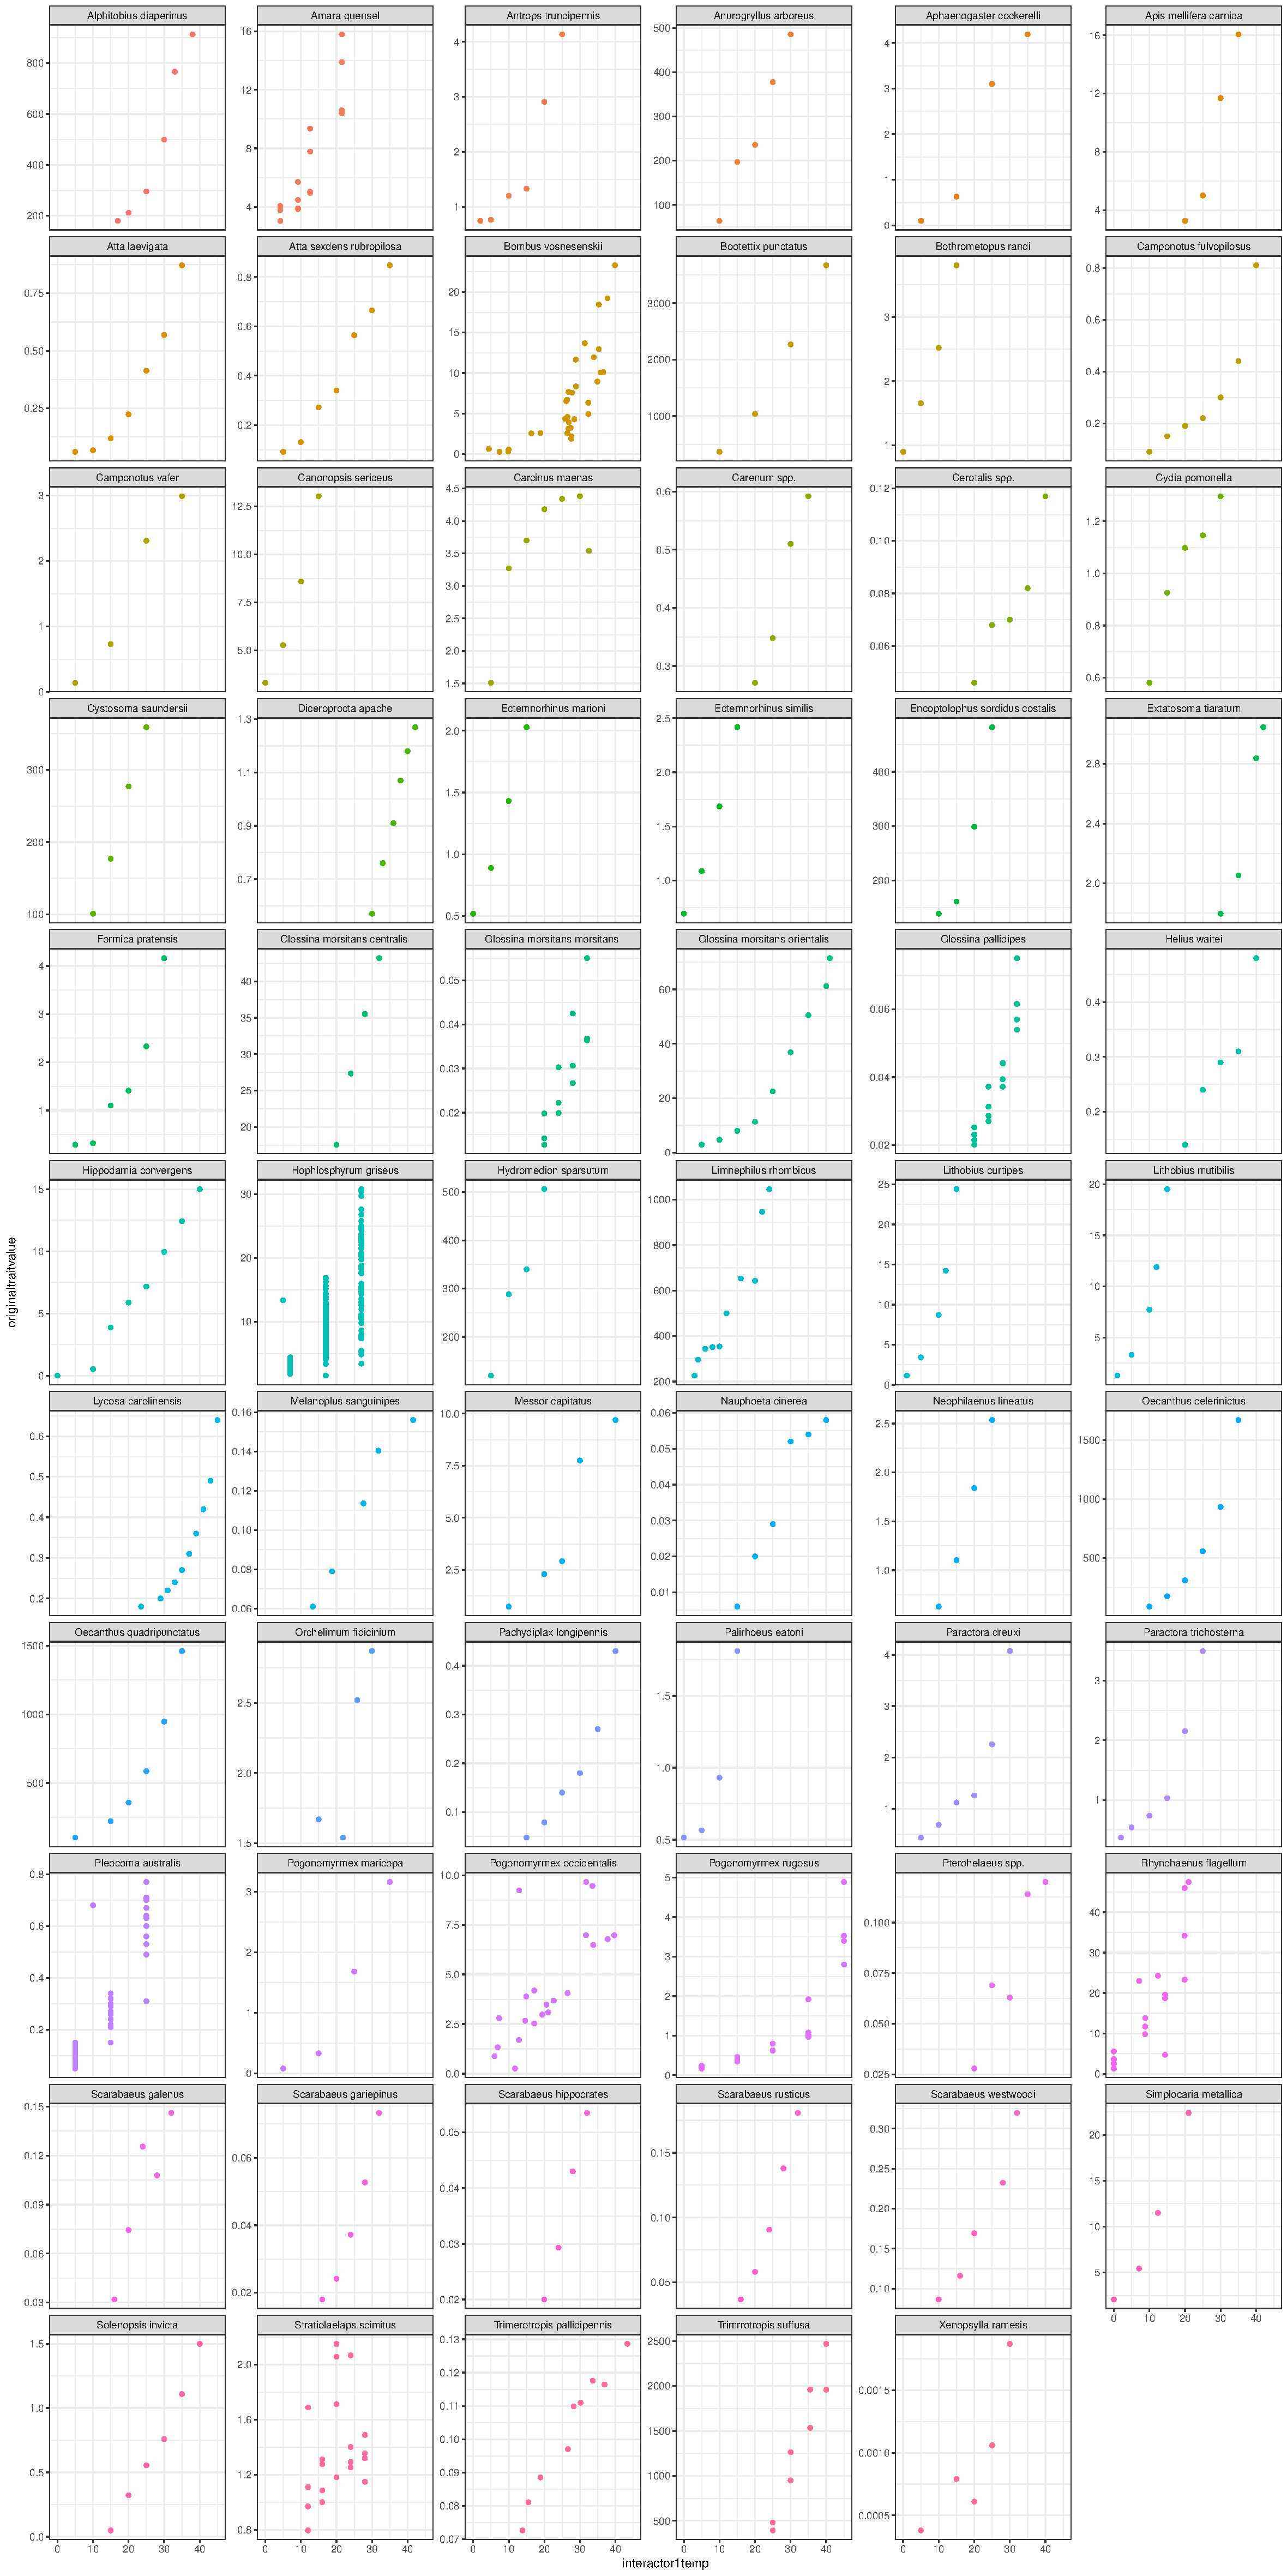
\includegraphics[width=3.43in]{AllMRs (2).pdf}
    \caption{\label{fig:11} Metabolic rate for each species. The x-axis is temperature and metabolic rate is the y-axis. Each plot corresponds to a different species}
\end{figure}
\clearpage

\section{Data Collection}
\begin{table}[h]
\tiny
\begin{tabular}{|l|l|}
\hline
\textbf{Study} & \textbf{DOI} \\ \hline
Bojrge et al. 2018. "Role of   temperature on growth \& metabolic rate...". J. Insect Physiol. 107 & 10.1016/j.jinsphys.2018.02.010 \\ \hline
Stromme et al. 1986. "Physiological   adaptations in Coleoptera on Spitsbergen". Polar Research 4 & 10.3402/polar.v4i2.6932 \\ \hline
Chown 1997. "Thermal sensitivity of   oxygen uptake of Diptera from sub-Antarctic…" Polar Biol 17:1 & 10.1007/s003000050108 \\ \hline
Prestwich \& Walker. 1981.   "Energetics of singing in crickets…". Journal of comparative   physiology. 143 & 10.1007/BF00797699 \\ \hline
Nielsen. 1986. "Respiratory rates of   ants from different climatic areas". Journal of Insect Physiology. 32:2 & 10.1016/0022-1910(86)90131-9 \\ \hline
Schmolz et al. 2002. "Calorimetric   investigations on metabolic rates...". Thermochimica Acta 382 & 10.1016/S0040-6031(01)00740-7 \\ \hline
Beraldo \& Mendes 1982. "The influence of temperature on oxygen…" Comp. Biochem. Physiol. A: Physiol 71:3 & 10.1016/0300-9629(82)90428-5 \\ \hline
Kammer \& Heinrich 1974.  "Metabolic rates related to muscle activity in bumblebees". JEB   61:1 & 10.1242/jeb.61.1.219 \\ \hline
Lozier et al. 2021. "Divergence in body mass wing loading \& population structure….". Insect Syst \&   Div 5:5 & 10.1093/isd/ixab012 \\ \hline
Mispagel. 1978. "The Ecology \& Bioenergetics of the Acridid Grasshopper...."   Ecology. 59:4. & 10.2307/1938782 \\ \hline
Klok \& Chown. 2005. "Temperature \& body mass related variation...". Insect Physiol. 51. & 10.1016/j.jinsphys.2005.03.007 \\ \hline
Lighton. 1989. "Individual \& Whole-Colony Respiration in an African Formicine Ant". Functional Ecology. 3:5. & 10.2307/2389566 \\ \hline
Halsey et al. "The interactions  between temperature \& activity levels …". 2014, Oecologia 177 & 10.1007/s00442-014-3190-5 \\ \hline
Duncan \& Dickman 2001.  "Respiratory patterns \& metabolism in tenebrionid…". Oecologia 129:4 & 10.1007/s004420100772 \\ \hline
van Hook 1971. "Energy \& Nutrient Dynamics of Spider \& Orthopteran…". Ecol. Monogr 41:1 & 10.2307/1942433 \\ \hline
Neven 1998. "Respiratory Response of   Fifth-Instar Codling Moth…". J Econ. Entomol. 91:1 & 10.1093/jee/91.1.302 \\ \hline
Boivin 2001. "Pleiotropy of   insecticide resistance in the codling moth..." Entomol. Exp. Appl. .99:3 & 10.1046/j.1570-7458.2001.00838.x \\ \hline
Mac Nally \& Doolan. 1982.   "Comparative Reproductive Energetics….".   Oikos. 39:2 & 10.2307/3544483 \\ \hline
Hadley et al. 1991. "Evaporative   Cooling in the Desert Cicada…". J. Exp. Biol. 159:1. & 10.1242/jeb.159.1.269 \\ \hline
Bailey \& Riegert 1973. "Energy   dynamics of Encoptolophus sordidus costalis…". Can. J. Zool. 51:1 & 10.1139/z73-014 \\ \hline
Hill 2019. "Impacts of temperature  on metabolic rates…". Physiol. Entomol.   45:1 & 10.1111/phen.12310 \\ \hline
Jensen \& Nielsen. 1975. "The   influence of body size \& temperature on worker ant respiration".   Nat. Jutl.. 18. & 10.1007/BF02229253 \\ \hline
Terblanche \& Chown 2007. "The   effects of temperature, body mass \& feeding…". Physiol. Entomol.   32:2 & 10.1111/j.1365-3032.2006.00549.x \\ \hline
Terblanche et al. 2005.   "Temperature-dependence of metabolic rate…". J. Insect Physiol. 51:8 & 10.1016/j.jinsphys.2005.03.017 \\ \hline
Rajagopal \& Bursell. 1965. "The   Respiratory Metabolism …". Journal of Insect   Physiology. 12:3 & 10.1016/0022-1910(66)90144-2 \\ \hline
Terblanche et al. 2009. "Directional  evolution of the slope…". Physiol. Biochem. Zool   82:5 & 10.1086/605361 \\ \hline
Terblanche et al. 2006. "Phenotypic   plasticity \& geographic variation…" Am J Trop   Med Hyg. 74:5 & 10.4269/ajtmh.2006.74.786 \\ \hline
Acar et al. 2001. "Use of  Calorespirometry to Determine Effects of Temperature...". Environ. Entomol. 30:5 & 10.1603/0046-225X-30.5.811 \\ \hline
Katsarou et al. 2005. "Effect of  temperature on development growth \& feeding …". BioControl   50:565Ð588 & 10.1007/s10526-004-2838-1 \\ \hline
Nespolo et al. 2003.   "Intrapopulational variation in the standard metabolic rate of insects …". Exp. Biol. 206. & 10.1242/jeb.00687 \\ \hline
Somme et al. 1989. "Respiratory  metabolism of Hydromedion sparsutum...".   Polar Biol. 10 & 10.1007/BF00239158 \\ \hline
Roux 1979. "The influence of some  ecological factors…". Freshw. Biol.   9:2 & 10.1111/j.1365-2427.1979.tb01495.x \\ \hline
Pennington \& Meehan 2007.   "Influence of Body Size \& Environmental Temperature…". Environ.   Entomol. 36:4 & 10.1093/ee/36.4.673 \\ \hline
Moeur \& Eriksen 1972. "Metabolic Responses to Temperature of a Desert Spider…"Physiol. Zool. 45:4 & 10.1086/physzool.45.4.30155585 \\ \hline
Chappel 1983. "Metabolism \& thermoregulation in desert \& montane grasshoppers". Oecologia  56:126-131. & 10.1007/BF00378228 \\ \hline
Nielsen \& Baroni Urbani. 1990.  "Energetics \& foraging behaviour of…".   Physiological Entomology. 15. & 10.1111/j.1365-3032.1990.tb00533.x \\ \hline
Schimpf et al. 2012. "Standard   metabolic rate is associated with gestation duration…". Biol. Open 1:12 & 10.1242/bio.20122683 \\ \hline
Hinton. 1971. "Energy Flow in a   Natural Population of Neophilaenus lineatus (Homoptera)". Oikos. 22:2. & 10.2307/3543722 \\ \hline
Smalley 1960. "Energy flow of a salt   marsh grasshopper" Pop. Ecol. 41:4 & 10.2307/1931800 \\ \hline
Lavy \& Verhoef 1996. "Effects of   food quality on growth \& body composition…". Physiol. Entomol. 21:1 & 10.1111/j.1365-3032.1996.tb00836.x \\ \hline
May. 1978. "Energy metabolism of   dragonflies ( Anisoptera)…". Exp. Biol. 83. & 10.1242/jeb.83.1.79 \\ \hline
Mercer et al. 2001. "Invertebrate   body sizes from Marion Island". Antarct. Sci. 13:2 & 10.1017/S0954102001000219 \\ \hline
Sustr \& Stary 1998. "Digestive   enzymes in oribatid mites...". Pedobiologia 38:250-253 & NA \\ \hline
Morgan. 1987. "Temp. Regulation   Energy Metabolism \& Mate-Searching…". Exp. Biol. 128:1. & 10.1242/jeb.128.1.107 \\ \hline
Rogers et al. 1972. "Bioenergetics   of the Western Harvester Ant…". Environ. Entomol. 1:6 & 10.1093/ee/1.6.763 \\ \hline
Ettershank \& Whitford. 1973.   "O2 of two species of Pogonomyrmex …". Comp.   Biochem. Physiol. 46:3. & 10.1016/0300-9629(73)90111-4 \\ \hline
Chown \& Davis. "Discontinuous  gas exchange \& the significance of respiratory water loss…". JEB   206:20 & 10.1242/jeb.00603 \\ \hline
Davis et al. 2000. "A comparative   analysis of metabolic rate in six Scarabaeus …" J. Insect. Physiol. 46:4 & 10.1016/S0022-1910(99)00141-9 \\ \hline
Elzen 1986. "Oxygen consumption  \& water loss in the imported fire ant…". Comp. Biochem. \&   Physiol. A: 84:1 & 10.1016/0300-9629(86)90035-6 \\ \hline
Meehan et al. 2022. "Predators  minimize energy costs rather than maximize energy gains". Funct.   Ecol. & 10.1111/1365-2435.14131 \\ \hline
Massion. 1983. "An altitudinal  comparison of water \& metabolic relations…". Comp Biochem Physiol.   74A:1 & 10.1016/0300-9629(83)90719-3 \\ \hline
Fielden et al. 2004.  "Respiratory gas exchange in the desert fle... ".   Comp. Biochem. Physiol. 137:3. & 10.1016/j.cbpb.2003.11.012 \\ \hline
\end{tabular}
\caption{\label{Table:S2} Table containing citation and DOI for each study included in the analysis. From these studies, metabolic rate data for 142 species from 48 families was measured across temperature ranges and collected along with information on life stage, experimental conditions, sex, body size, location and accumilation temperature}
\end{table}


\clearpage
\bibliographystyle{plainnat}
\bibliography{proj}
\end{document}
